\documentclass[12pt,a4paper]{article}
\usepackage{amsmath}
\usepackage{amsfonts}
\usepackage{amssymb}
\usepackage{graphicx}
\usepackage{secdot}
\usepackage[left=2cm,right=2cm,top=2cm,bottom=2cm]{geometry}

\author{ Shibayan Biswas, AE21B109\\ Department of Aerospace Engineering\\ IIT Madras\\[3ex] Instructor:\\ \large Professor Dr. Manikandan Mathur}

\title{Experiment- 4}

\date{September 21, 2022}

\begin{document}

\maketitle
\hline
\section{Aim:}
To calibrate a Bordon Type Pressure Gauge, to establish calibration curve for Bordon Type Pressure Gauge and to determine the Errors in the Bordon Type Pressure Gauge along with minimising them.
\section{Introduction:}
Instrument calibration is one of the primary processes used to maintain instrument accuracy. It is the process of configuring an instrument to provide results within an acceptable range. Known weights have been applied on a Dead Weight Calibrator to apply pressure to a fluid for checking the accuracy of readings from a pressure gauge. Various types of pressure measuring instrument have been used to measure the pressure intensity at any point in static or moving fluid. One of these devices is the
Bordon tube pressure gauge. Bordon-tube pressure gauges are most widely used now-days because of their reliability, compactness, low cost and ease of use. It consists of a curved tube (Figure 1) of elliptical cross-section bent into a circular arc. \\
\\When pressure is applied to the tube, it tends to straighten out, and the deflection of the end of the tube is communicated through a system of levers to a recording pointer. This gauge is widely used for steam and compressed gases. The pressure indicated is the difference between the system pressure and to the external (ambient) pressure, and is usually referred to as the gauge pressure. 
\clearpage
\begin{figure}[!ht]
	\begin{center}
			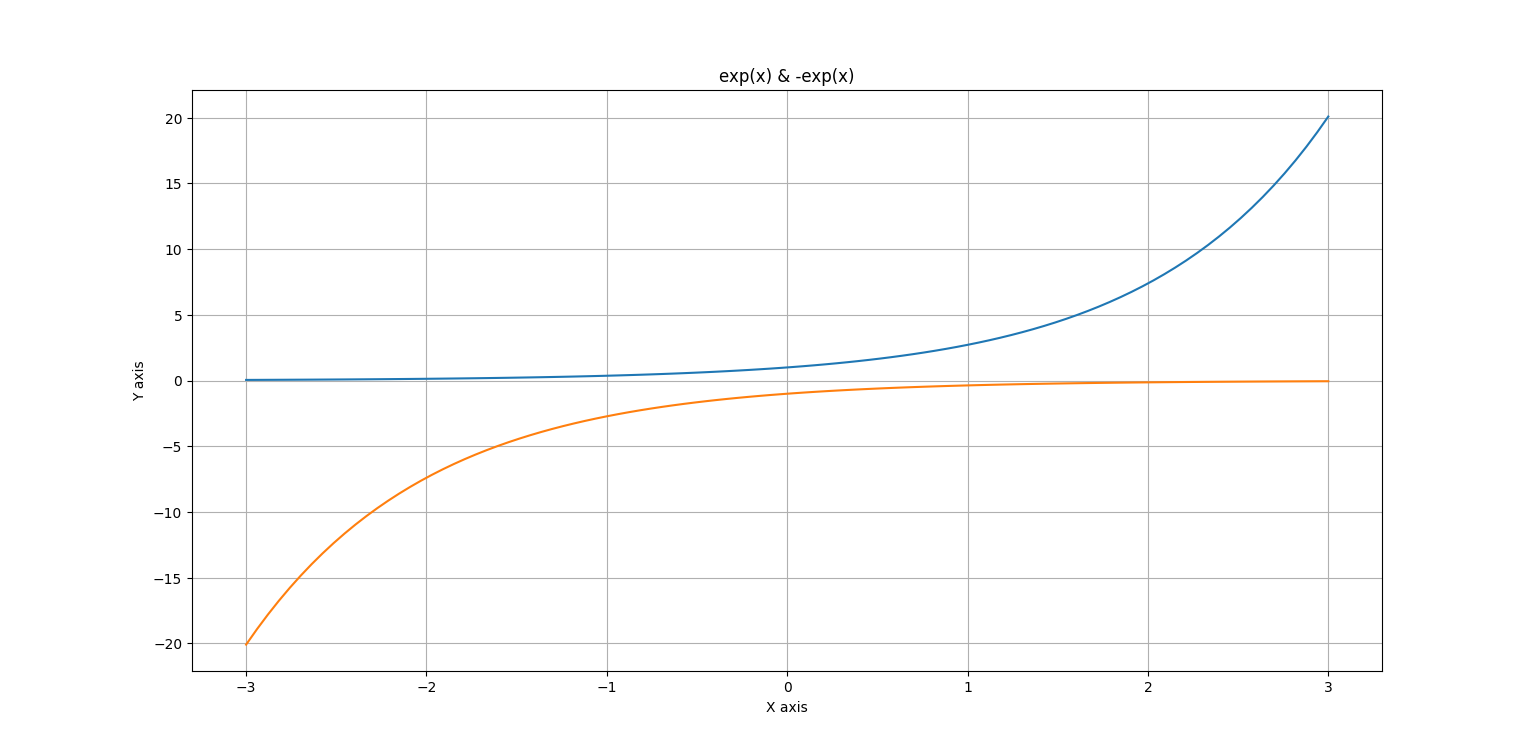
\includegraphics[scale=0.8]{Figure_1.png}
	\end{center}
	\caption{Dead Weight Calibrator}
\end{figure}
\section{Equipment:}
The following equipment were required to perform the particular experiment. They are shown below:
\begin{itemize}
\item Bordon pressure gauge
\item Dead Weight Calibrator
\item Set of Test weights
\item Weight balance
\end{itemize}
\section{Theory:}
The Bordon Gauge is the most popular pressure measuring device for both liquids and gasses. It can be connected to any source of pressure such as a pipe or vessel containing a pressurized fluid. 
\subsection{Bordon Gauge:}
The Bordon Gauge (Figure 2) is fitted with a transparent dial, which lets you see the internal workings of the gauge. The gauge consists of a thin walled closed ended tube which is oval in cross section. This tube is bent through an angle of about 270o along its long axis. The open end of the tube is welded to a hollow mounting block which allows the pressurized fluid to reach the tube. This causes the pressure from the source to be transmitted directly to the inside of the Bordon tube. The applied pressure causes the oval tube to become rounder (since a round cross section has the maximum area for a given circumference). As it becomes rounder, the Bordon tube tends to uncurl which causes its free end to move. A system of linkages and levers transmits this motion to the gauge needle which moves over the scale.
\begin{figure}[!ht]
	\begin{center}
			
\includegraphics[scale=0.09]{Figure_2.jpg}
	\end{center}
	\caption{Bordon Gauge }
\end{figure}\
\subsection{Dead Weight Calibrator:}
In order to obtain very accurate pressure measurements, it is essential to regularly re-calibrate the gauge. This is because the tube tends to become weaker with extended use. The usual procedure is to apply a known pressure to the gauge using a device called a Dead Weight Calibrator. The normal calibration procedure is to load the gauge for known pressures, using a dead weight calibrator including a liquid of known specific gravity (use water as the liquid). This dead weight tester uses a simple piston and cylinder arrangement to provide a source of pressurized liquid (in the experiment water will produced a better result than oil) which is transmitted to the gauge. Since the true pressure of the liquid can be easily calculated, the value can be compared directly to the reading on the gauge over the complete scale range. (The scale range is the range of pressures from zero to the full-scale deflection value). The dead weight tester consists of a cylindrical piston which is free to move vertically in a close fitting cylinder. \\
\\A Platen is attached to the piston which can be loaded with a series of accurate weights. The pressure developed in the cylinder is transmitted via a transparent tube to the gauge under test. The cylinder is mounted on a base board which is supported on leveling screws and fitted with a spirit level.\\
\subsection{Theoretical Equations:}
The use of the piston and weights with the cylinder generates a measurable reference pressure: 
\begin{equation}
\text{P} = \frac{\text{F}}{\text{A}}
\end{equation}
\begin{equation}
\text{F} = \text{M} \text{g}
\end{equation}
F = Force applied to the liquid in the calibrator cylinder in Newton (N)\\
M = Total mass including the mass of the piston in kilogram (kg)\\
A = Cross-sectional area of the piston in square meter ($m^2$)\\
g = Acceleration due to gravity in meter per square second ($m/s^2$)\\
\section{Experimental Setup:}
\begin{itemize}
\item Position the calibrator without the piston on the hydraulic bench top and ensure that the base is horizontal by adjusting the feet and using the spirit level. This is necessary to ensure vertical transfer of the applied load and free rotation of the piston. 
\item Open all cocks on the pressure gauge base. 
\item Connect the inflow cock to the bench flow connector and the outflow cock to the lower tube from the calibrator cylinder.
\item Open slowly the bench valve to produce a flow, tilt the pressure gauge to ensure that air is driven out from the manifold and then close the middle cock on the manifold. 
\item When there is no further air emerging and the calibrator cylinder is full, close the bench valve and the inflow cock on the manifold. 
\end{itemize}
\section{Procedure:}
\begin{itemize}
\item Measure the weight of the calibration masses. 
\item Note down the weight of the piston and it’s cross sectional area.
\item Remove the piston and pour the water into the cylinder until it is full to overflow level. Any air trapped in the tube may be cleared by tilting and gently tapping the apparatus. 
\item Insert the piston carefully and spin it to minimize any friction effects. 
\item Note the pressure reading from the gauge. 
\item Add the weights in convenient increments, and at each increment, observe the pressure gauge reading. 
\item Take the similar sets of readings with decreasing weights. 
\end{itemize}
Note : If due to the slight leakage, piston reaches the cylinder bottom, more water must be added to the cylinder.
\section{Results:}
The tables representing the experimental and the theoretical values along with the plots showing the variation of the respective values for the following experiment is provided in this section:\\
\\Weight of Cylinder = 0.5 Kg\\
Diameter of Cylinder = 17.67 mm\\
Initial Error in Bordon Gauge = 15 $KN/m^2$\\
\begin{table}[!ht]
\begin{center}
\begin{tabular}{|p{2cm}|p{2cm}|p{6cm}|p{6cm}|}
\hline
Serial No. & Weight(kg) & Pressure while loading(KPa) & Pressure while unloading(KPa) \\
\hline
1 & 0.5 & 29 & 35\\
2 & 0.5 & 32 & 34\\
3 & 0.5 & 35 & 34\\
4 & 0.5 & 33 & 32\\
5 & 0.5 & 34 & 35\\
\hline
\end{tabular}
\caption{Raw Data Table when weight is 0.5 kg}
\end{center}
\end{table}
\begin{table}[!ht]
\begin{center}
\begin{tabular}{|p{2cm}|p{2cm}|p{6cm}|p{6cm}|}
\hline
Serial No. & Weight(kg) & Pressure while loading(KPa) & Pressure while unloading(KPa) \\
\hline
1 & 1.0 & 50 & 52\\
2 & 1.0 & 58 & 54\\
3 & 1.0 & 52 & 54\\
4 & 1.0 & 52 & 54\\
5 & 1.0 & 52 & 55\\
\hline
\end{tabular}
\caption{Raw Data Table when weight is 1 kg}
\end{center}
\end{table}
\begin{table}[!ht]
\begin{center}
\begin{tabular}{|p{2cm}|p{2cm}|p{6cm}|p{6cm}|}
\hline
Serial No. & Weight(kg) & Pressure while loading(KPa) & Pressure while unloading(KPa) \\
\hline
1 & 1.5 & 84 & 74\\
2 & 1.5 & 80 & 75\\
3 & 1.5 & 73 & 75\\
4 & 1.5 & 73 & 74\\
5 & 1.5 & 72 & 74\\
\hline
\end{tabular}
\caption{Raw Data Table when weight is 1.5 kg}
\end{center}
\end{table}
\begin{table}[!ht]
\begin{center}
\begin{tabular}{|p{2cm}|p{2cm}|p{6cm}|p{6cm}|}
\hline
Serial No. & Weight(kg) & Pressure while loading(KPa) & Pressure while unloading(KPa) \\
\hline
1 & 2.5 & 119 & 114\\
2 & 2.5 & 120 & 115\\
3 & 2.5 & 112 & 114\\
4 & 2.5 & 112 & 113\\
5 & 2.5 & 111 & 113\\
\hline
\end{tabular}
\caption{Raw Data Table when weight is 2 kg}
\end{center}
\end{table}
\clearpage
\begin{table}[!ht]
\begin{center}
\begin{tabular}{|p{2cm}|p{2cm}|p{6cm}|p{6cm}|}
\hline
Serial No. & Weight(kg) & Pressure while loading(KPa) & Pressure while unloading(KPa) \\
\hline
1 & 5.0 & 181 & 181\\
2 & 5.0 & 188 & 188\\
3 & 5.0 & 189 & 189\\
4 & 5.0 & 186 & 186\\
5 & 5.0 & 187 & 187\\
\hline
\end{tabular}
\caption{Raw Data Table when weight is 2.5 kg}
\end{center}
\end{table}
\begin{table}[!ht]
\begin{center}
\begin{tabular}{|p{2cm}|p{2cm}|p{6cm}|p{6.5cm}|}
\hline
Serial No. & Weight(Kg) & Experimental Pressure (loading) & Experimental Pressure (unloading)\\
\hline
1 & 0.5 & 17.6 & 19\\
2 & 1.0 & 37.8 & 38.8\\
3 & 1.5 & 61.4 & 59.4\\
4 & 2.5 & 99.8 & 98.8\\
5 & 5.0 & 171.2 & 171.2\\
\hline
\end{tabular}
\caption{Raw Data Table for experimental Pressures}
\end{center}
\end{table}
\begin{table}[!ht]
\begin{center}
\begin{tabular}{|p{2cm}|p{2.5cm}|p{5cm}|}
\hline
Serial No. & Weight(Kg) & Theoretical Pressures(KPa)\\
\hline
1 & 0.5 & 19.9\\
2 & 1.0 & 39.9\\
3 & 1.5 & 59.9\\
4 & 2.5 & 99.9\\
5 & 5.0 & 199.9\\
\hline
\end{tabular}
\caption{Raw Data Table for Theoretical Pressures}
\end{center}
\end{table}
\clearpage
\begin{figure}[!ht]
	\begin{center}
	    \framebox{
			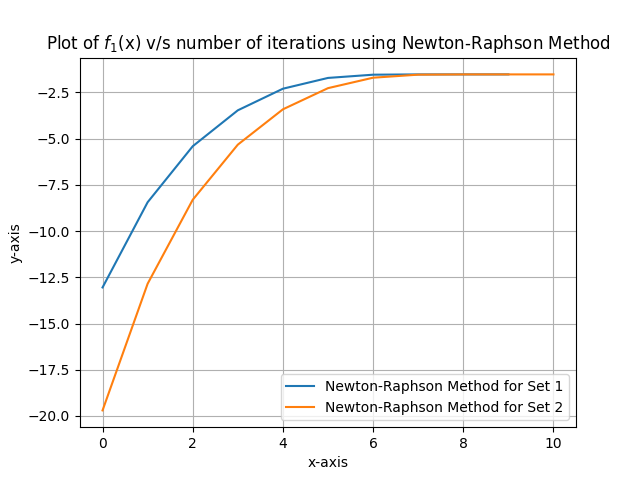
\includegraphics[scale=0.8]{Figure_3.png}
		}
	\end{center}
\end{figure}
\begin{itemize}
\item The figure above shows the scatter plot for the data values obtained and the best-fit line that passes through the origin y = mx. The value of m = 0.887.
\item Expected m = 1. Error in m, e = 0.113.
\end{itemize}
\begin{figure}[!ht]
	\begin{center}
	    \framebox{
			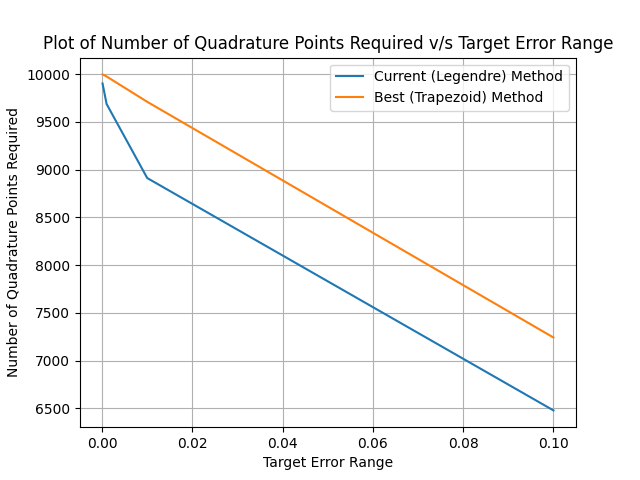
\includegraphics[scale=0.8]{Figure_4.png}
		}
	\end{center}
\end{figure}
\begin{itemize}
\item The figure above shows the scatter plot for the data values obtained and the best-fit line that passes through the origin y = mx. The value of m = 0.919.
\item Expected m = 1. Error in m, e = 0.081.
\end{itemize}
\begin{figure}[!ht]
	\begin{center}
	    \framebox{
			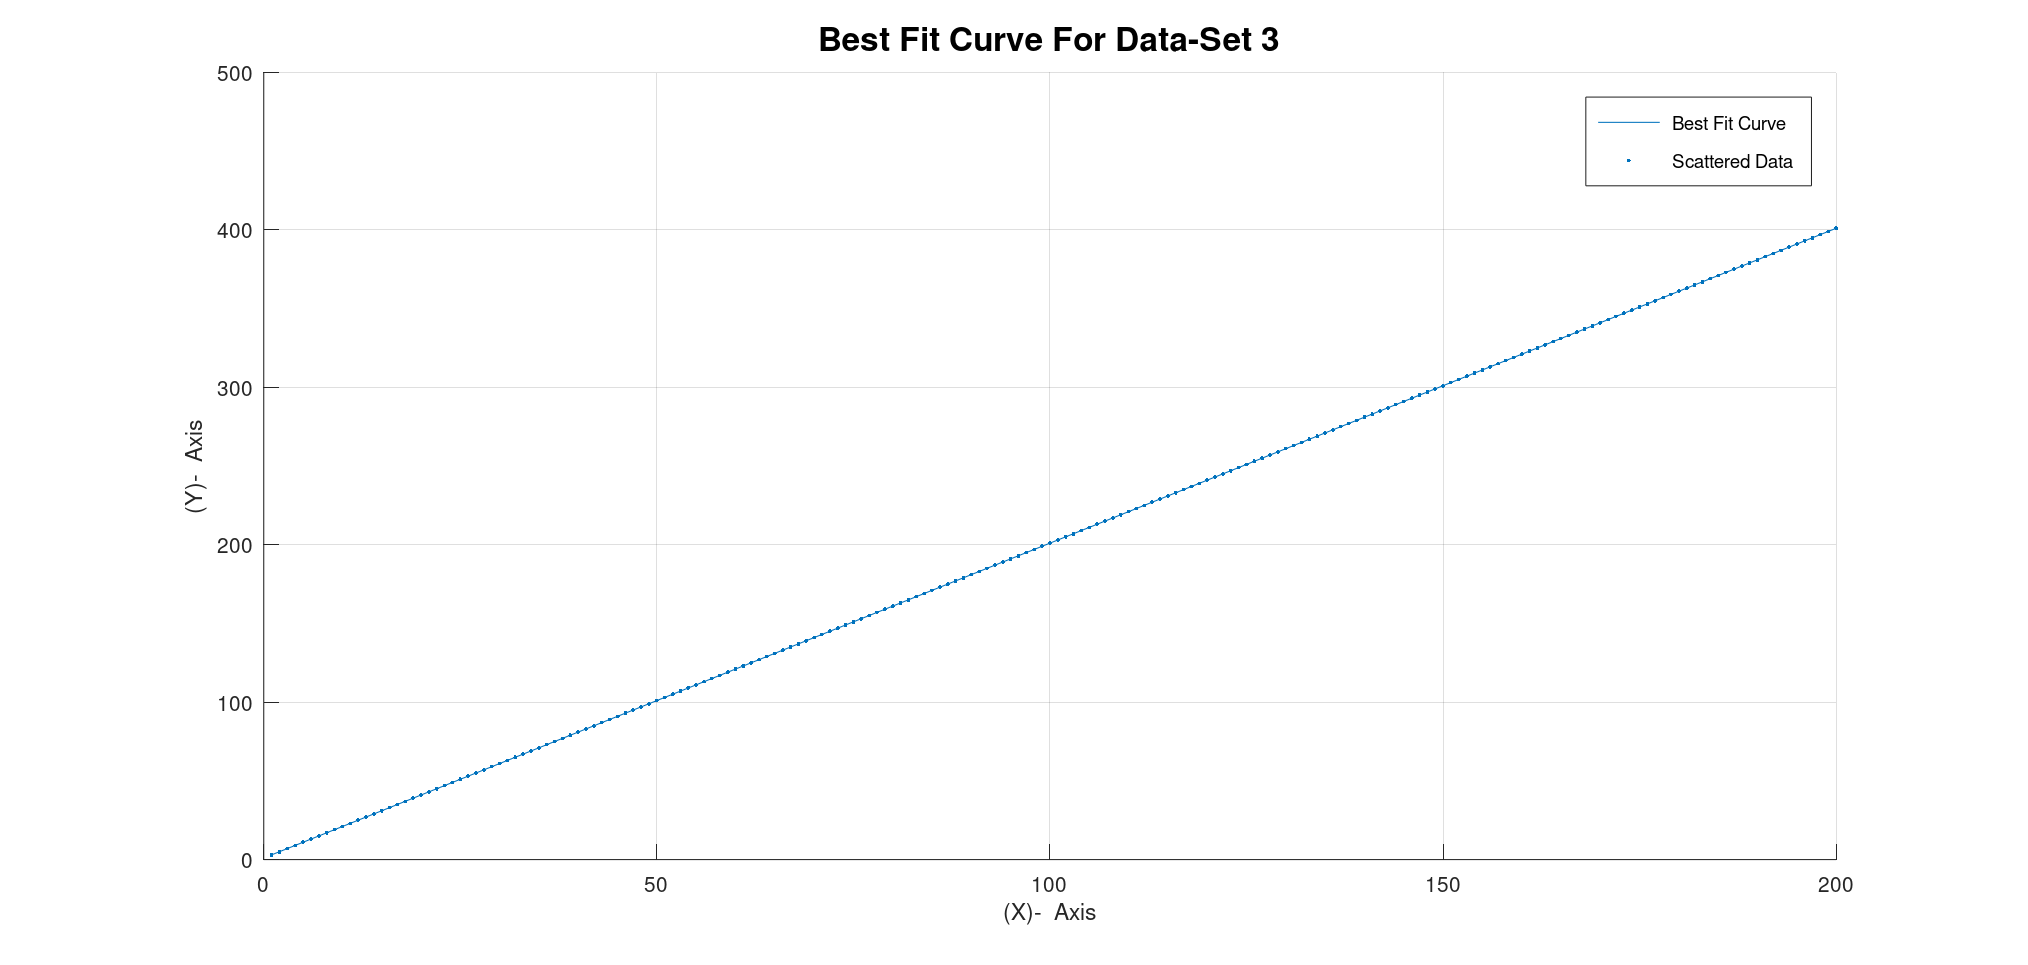
\includegraphics[scale=0.8]{Figure_5.png}
		}
	\end{center}
\end{figure}
\begin{itemize}
\item The figure above shows the scatter plot for the data values obtained and the best-fit line that passes through the origin y = mx. The value of m = 0.908.
\item Expected m = 1. Error in m, e = 0.092.
\end{itemize}
\clearpage
\begin{figure}[!ht]
	\begin{center}
	    \framebox{
			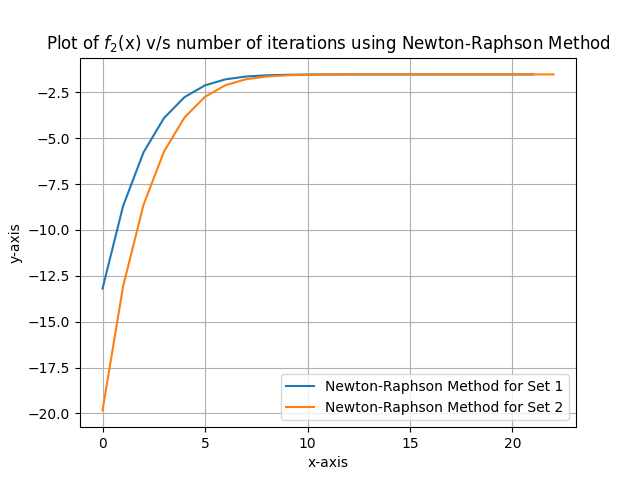
\includegraphics[scale=0.8]{Figure_6.png}
		}
	\end{center}
\end{figure}
\begin{itemize}
\item The figure above shows the scatter plot for the data values obtained and the best-fit line that passes through the origin y = mx. The value of m = 0.894.
\item Expected m = 1. Error in m, e = 0.106.
\end{itemize}
\begin{figure}[!ht]
	\begin{center}
	    \framebox{
			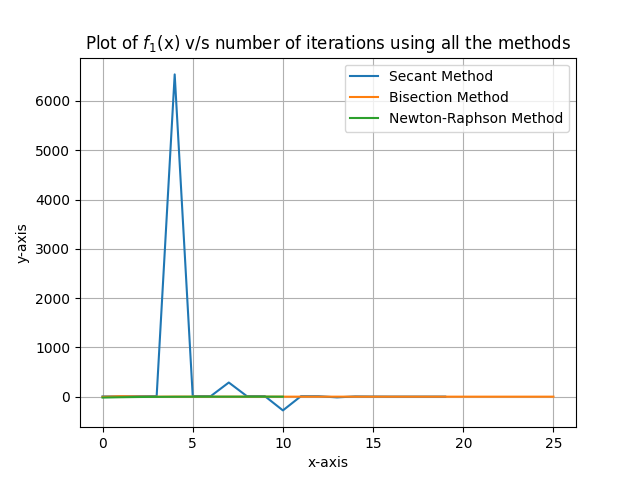
\includegraphics[scale=0.8]{Figure_7.png}
		}
	\end{center}
\end{figure}
\begin{itemize}
\item The figure above shows the scatter plot for the data values obtained and the best-fit line that passes through the origin y = mx. The value of m = 0.898.
\item Expected m = 1. Error in m, e = 0.102.
\end{itemize}
\section{Sources of Error:}
From the data obtained through the experiments, we can conclude that the Bordon Gauge is an extremely helpful pressure measurement device which can be used for applications where minor errors are admissible.\\
Using the mean values the error \% = e × 100 = 10 \% \\
Any deviations in values could be due to the errors listed below:\\
\begin{itemize}
\item Errors due to hysteresis. Hysteresis is a measure of how effective a pressure gauge is in repeating the upscale reading on the downscale cycle under the same conditions.
\item Corrosion of the tube.
\item Vibrations and over-pressure.
\item Error in taking readings.
\item Approximations in values taken and low precision of the instrument.
\item Variations in experimental conditions.
\item Assumptions made are not strictly satisfied.
\end{itemize}
\section{Conclusion:}
We can conclude that the pressure measurement using a Bordon Gauge is fairly accurate and advantageous for applications that allow an error of about 10 \%. Any deviations from theoretically expected values can be reduced by greater care in taking readings.
\end{document}